\documentclass[UTF8,a4paper,12pt]{ctexbook} 

\usepackage{graphicx}%学习插入图
\usepackage{verbatim}%学习注释多行
\usepackage{booktabs}%表格
\usepackage{geometry}%图片
\usepackage{amsmath}
\usepackage{amssymb}
\usepackage{listings}%代码
\usepackage{xcolor}  %颜色
\usepackage{enumitem}%列表格式
\setenumerate[1]{itemsep=0pt,partopsep=0pt,parsep=\parskip,topsep=5pt}
\setitemize[1]{itemsep=0pt,partopsep=0pt,parsep=\parskip,topsep=5pt}
\setdescription{itemsep=0pt,partopsep=0pt,parsep=\parskip,topsep=5pt}
\usepackage{tcolorbox}
\usepackage{algorithm}  %format of the algorithm
\usepackage{algorithmic}%format of the algorithm
\usepackage{multirow}   %multirow for format of table
\usepackage{tabularx} 	%表格排版格式控制
\usepackage{array}	%表格排版格式控制
\usepackage{hyperref} %超链接 \url{URL}
\usepackage{tikz}
\usepackage{dirtree}

\CTEXsetup[format+={\flushleft}]{section}

%%%% 设置图片目录
\graphicspath{{figure/}}

%%%% 段落首行缩进两个字 %%%%
\makeatletter
\let\@afterindentfalse\@afterindenttrue
\@afterindenttrue
\makeatother
\setlength{\parindent}{2em}  %中文缩进两个汉字位

%%%% 下面的命令重定义页面边距,使其符合中文刊物习惯 %%%%
\addtolength{\topmargin}{-54pt}
\setlength{\oddsidemargin}{0.63cm}  % 3.17cm - 1 inch
\setlength{\evensidemargin}{\oddsidemargin}
\setlength{\textwidth}{14.66cm}
\setlength{\textheight}{24.00cm}    % 24.62

%%%% 下面的命令设置行间距与段落间距 %%%%
\linespread{1.4}
\setlength{\parskip}{0.5\baselineskip}
\geometry{left=1.6cm,right=1.8cm,top=2cm,bottom=1.7cm} %设置文章宽度
\pagestyle{plain} 		  %设置页面布局

%代码效果定义
\definecolor{mygreen}{rgb}{0,0.6,0}
\definecolor{mygray}{rgb}{0.5,0.5,0.5}
\definecolor{mymauve}{rgb}{0.58,0,0.82}
\lstset{ %
	backgroundcolor=\color{white},   % choose the background color
	basicstyle=\footnotesize\ttfamily,      % size of fonts used for the code
	%stringstyle=\color{codepurple},
	%basicstyle=\footnotesize,
	%breakatwhitespace=false,         
	%breaklines=true,                 
	%captionpos=b,                    
	%keepspaces=true,                 
	%numbers=left,                    
	%numbersep=5pt,                  
	%showspaces=false,                
	%showstringspaces=false,
	%showtabs=false,        
	columns=fullflexible,
	breaklines=true,                 % automatic line breaking only at whitespace
	captionpos=b,                    % sets the caption-position to bottom
	tabsize=4,
	commentstyle=\color{mygreen},    % comment style
	escapeinside={\%*}{*)},          % if you want to add LaTeX within your code
	keywordstyle=\color{blue},       % keyword style
	stringstyle=\color{mymauve}\ttfamily,     % string literal style
	frame=single,
	rulesepcolor=\color{red!20!green!20!blue!20},
	% identifierstyle=\color{red},
	language=c++,
}
 \author{\kaishu 郑华}
 \title{\heiti 音乐笔记}
 
\begin{document}          %正文排版开始
 	\maketitle
 
\chapter{看谱唱歌、乐理基础}
	\section{音名、唱名、音符、休止符、拍号}
	 	常用符号表示记号:\url{https://blog.csdn.net/chuchus/article/details/46042673}
	 	
		\subsection*{唱名、音名、级音、属名}
		 	
		 	\begin{table}[H]
		 		\centering
		 		\caption{音名唱名等对应表}
		 		\begin{tabular}{c|c|c|c|c|c|c|c}
		 		\toprule
		 			简谱 & 1 		& 2 & 3 & 4 & 5 & 6 & 7 \\
		 		\midrule
		 			音名 & C 		&D 	&E& F &G &A &B \\
		 			唱名 & Do 	&Re &Mi &Fa &Sol& La& Si \\
		 			级音 & 1级音  	& 2级音 & 3级音 & 4级音 & 5级音 & 6级音 & 7级音\\
		 			属名 & 主音 	& 上主音 &中音 & 下属音 & 属音 & 下中音 & 导音\\
		 		\bottomrule
		 		\end{tabular}
		 	\end{table}
		
		
		\subsection*{音组}
			\begin{figure}[H]
				\centering
				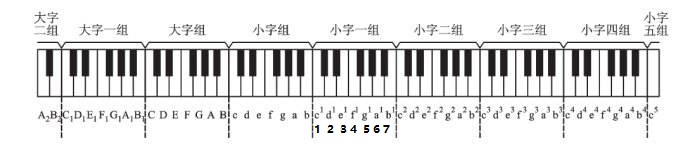
\includegraphics[width=16cm]{yinzu}
				\caption{音组示例}
			\end{figure}	
		
			小字一组对应 1,2,3,4,5,6,7 
	 
		\subsection*{音符、休止符}
			
			全音符、  2分、  4分、   8分、  16分、  32分。具体的是1对2的关系,一个全音符等于两个2分音符,以此类推。
		
			\begin{figure}[H]
				\centering
				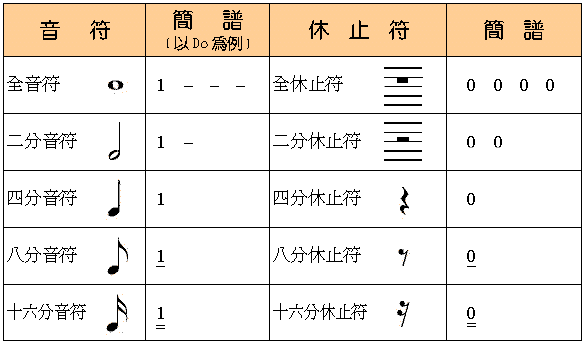
\includegraphics[width=15cm,height=8cm]{yinfu}
				\caption{音符与休止符表示记号}
			\end{figure}
			
		\subsection*{拍号(拍子记号)}
			$\dfrac{\textbf{每小节有几拍}}{\textbf{x分音符当1拍}} $,如$\dfrac{3}{4} $(每小节有3拍,每个4分音符当一拍)、  $\dfrac{2}{2} $ (每小节有2拍,每个2分音符当一拍)等.
		
		\subsection*{节拍}
			一个8分音符(\underline{x})为半拍,记为\verb|\| 或者 \verb|/|
		
			一个四分音符(\verb|x|)为一拍, 记为\verb|\/ 大|

			一个二分音符(\verb|x-|)记为两拍,记为\verb|\/ \/ 大大|
			
			一个全音符(\verb|x---|)记为4拍,记为\verb|\/ \/ \/ \/ 大大大大|	
			
					
		\subsection*{半音}
			只有 3-4,7-$\hat{1}$ 是半音。
			
			对应于钢琴上的相邻键。
			
			对应于吉他上的相邻品。
			
			\begin{figure}[H]
				\centering
				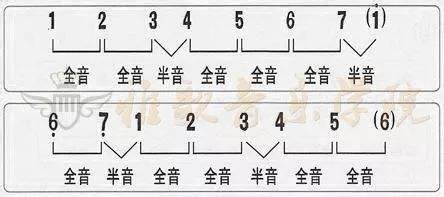
\includegraphics[width=15cm,height=3cm]{timg.jpg}
				\caption{全音半音演示}
			\end{figure}
			
			
		\subsection*{反复记号,附点音符}
			\begin{figure}[H]
				\centering
				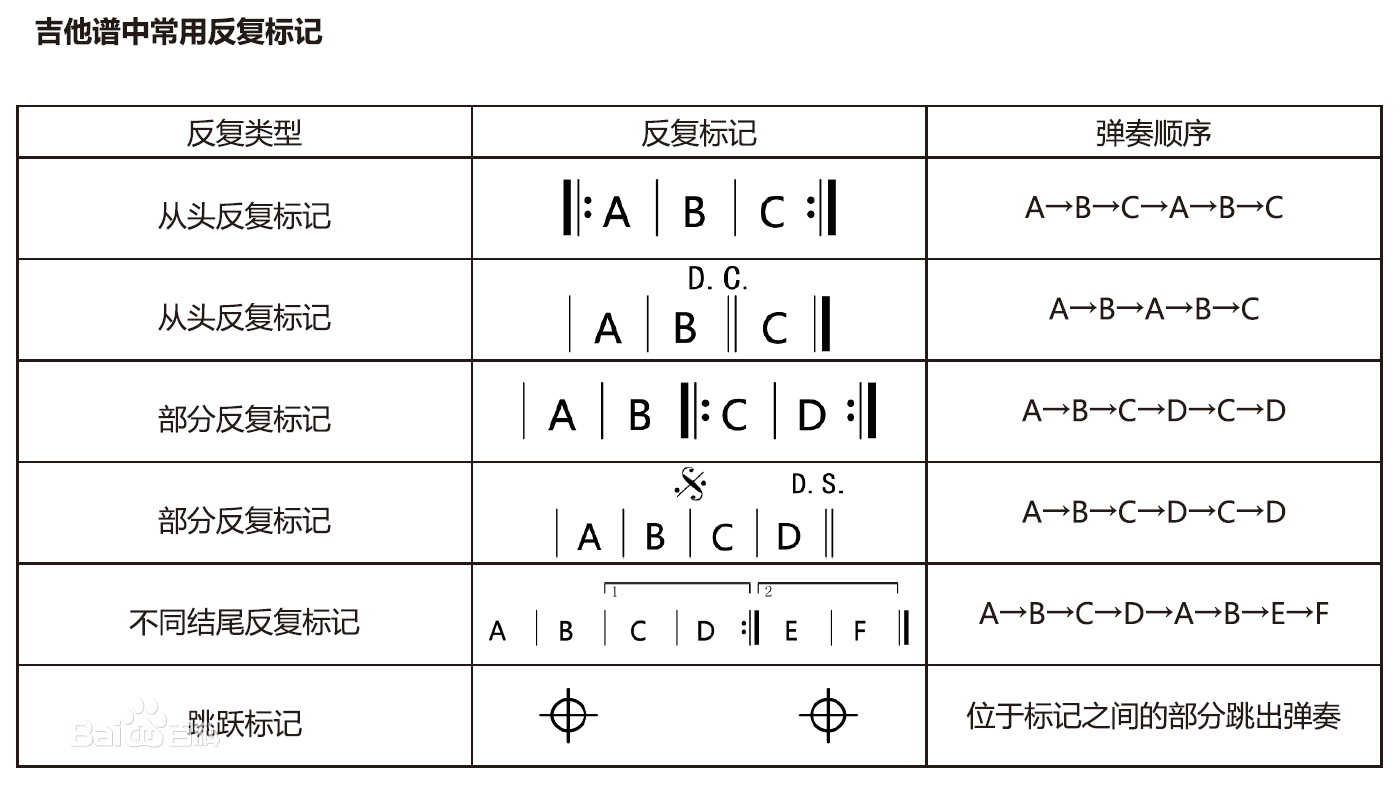
\includegraphics[scale=0.34]{repeat}
				\caption{重复标记}
			\end{figure}
			
		\newpage
		\subsection*{音程}
			用“度”来表示。
			
			\begin{figure}[H]
				\centering
				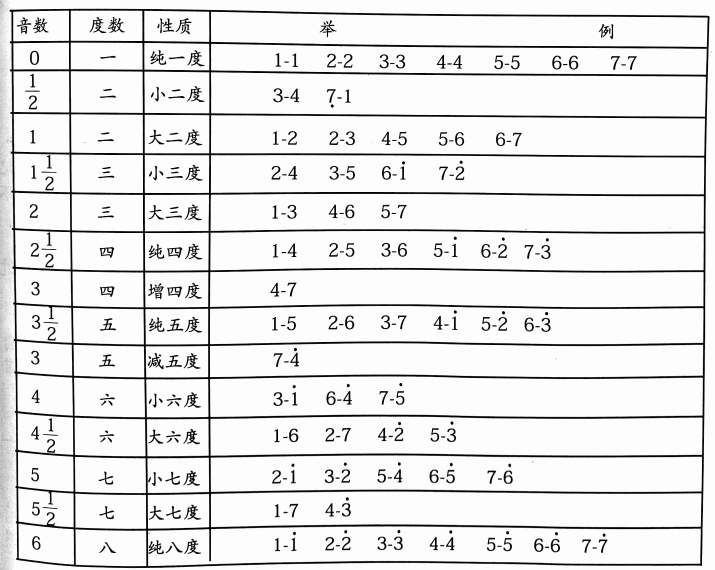
\includegraphics[width=0.97\linewidth]{figure/yincheng}
				\caption{音程示例}
				\label{fig:yincheng}
			\end{figure}
			
			口诀:“\textit{一四五八无大小,二三六七没有纯}”。
			
			\paragraph{协和音程}欢快、明亮
				\begin{itemize}[itemindent = 1em]
					\item \textbf{极协和音程}(纯1度(1-1)、纯8度(1-$\hat{1}$))
					\item \textbf{完全协和音程}(纯4度(1-4)、纯5度(1-5))
					\item \textbf{不完全协和音程}(大三小三度、大6小6度)
				\end{itemize}
				
			
			
			\paragraph{非协和音程}悲伤、紧张
				\begin{itemize}[itemindent = 1em]
					\item 大2、小7
					\item 小2、大7
					\item 增4、减5音程
				\end{itemize}
		
		
		\subsection{和弦}
			由三个或三个以上的音按照一定的音程关系叠加构成的一种组合方式。	
			
			\paragraph{3和弦}
				由三个音按照三度音程叠加构成, 以根音的名称来命名。
				
				\begin{figure}[H]
					\centering
					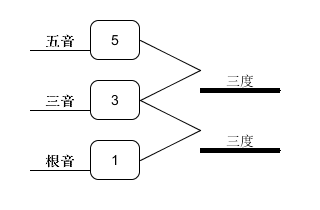
\includegraphics[height=6cm]{sanhexian}
					\caption{三和弦构成与名称}
				\end{figure}
				
				常用的三和弦有以下4种:
				\begin{itemize}[itemindent = 1em]
					\item \textbf{大三和弦}:根音与三音音程为大三度、三音与五音音程为小三度
					\item \textbf{小三和弦}:根音与三音音程为小三度、三音与五音音程为大三度
					\item \textbf{增三和弦}:根音与三音,三音与五音都是大三度
					\item \textbf{减三和弦}:根音与三音,三音与五音都是小三度
				\end{itemize}
			
			
			\paragraph{7和弦}
				由四个音按三度叠置而成的一种和弦,其显著特点是 根音(最低音)与冠音(最高音)音相距为七度,故名七和弦,其不协和性及紧张度来自七音。
				
				\begin{figure}[H]
					\centering
					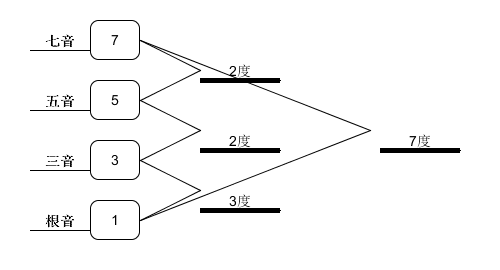
\includegraphics[height=6cm]{7hexian}
					\caption{7 和铉构成与名称}
				\end{figure}
				
				七和弦共有七类
				\begin{itemize}[itemindent = 1em]
					\item \textbf{大小七和弦}:以大三和弦为基础,根音与七音相距为小七度的和 弦。因为在和声大小调、自然大调旋律小调中常常以属音作为根音,因此它也称为属七和弦。
					\item \textbf{大七和弦}:以大三和弦为基础,根音与七音相距为大七度的和弦。
					\item \textbf{小七和弦}:以小三和弦为基础,根音与七音相距为小七度的和弦。
					\item \textbf{小大七和弦}:以小三和弦为基础,根音与七音相距为大七度的和弦。
					\item \textbf{减七和弦}:以减三和弦为基础,根音与七音相距为减七度的和弦。
					\item \textbf{减小七和弦}(半减七和弦):以减三和弦为基础,根音与七音相距为小七度的和弦。因为它经常以导音作为根音,所以它也称为导七和弦。
					\item \textbf{增小七和弦}:以增三和弦为基础,根音与七音相距为小七度的和弦。
					\item \textbf{增大七和弦}:以增三和弦为基础,根音与七音相距为大七度的和弦。
				\end{itemize}
			
			
			\paragraph{5和弦-万能和弦}
				就是原位三和弦,\textbf{省略三音}的和弦
				
				如\textit{1 3 5} 省略 3 后 \textit{1 5} , 也就是C5和弦 (根音为C)
			
			
		\subsection{调式}
			\textbf{以一个音为主音(第1音,起音)},按照一定的音程度数关系排列起来形成的音列。	
	
			\textbf{大调} 1234567 的半音全音间隔 如上,既 \textbf{全全半全全全半}, 音感\textit{比较欢快}。\textit{以1为主音}
			
			\textbf{小调} 1234567 的半音全音间隔 的排列为:\textbf{ 全半全全半全全}, 音感\textit{比较忧伤}。\textit{以6为主音}
			
			还有就是常看到谱上有什么C调E调(\textit{起音})之类的是什么意思:
			
			\begin{itemize}[itemindent = 1em]
				\item 1 2 3 4 5 6 7 $\hat{1}$ C大调 以1(C)音为调起唱
				\item 5 6 7 1 2 3 \#4 5 G大调 以5(G)音为调起唱
			\end{itemize}
		
			\textbf{变调夹}的作用就是不改变指法变调,既如果是D调,则夹1品,从2品用C调的指法弹就好了。	
	
	\newpage
	\section{吉他常用和弦}
	
		 \verb|A A7 Am Am7|
		
		 \verb|B7 Bm Bm7| 
		 
		 \verb|C C7| 
		 
		 \verb|D D7 Dm Dm7 |
		 
		 \verb|E E7 Em| 
		 
		 \verb|F Fmaj7| 
		 
		 \verb|G G7 | 
	
			\begin{figure}[H]
				\centering
				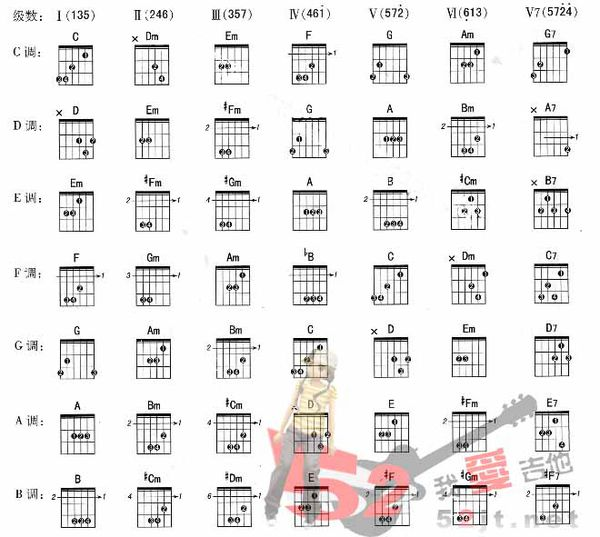
\includegraphics[width=17cm,height=15cm]{hexuan}
				\caption{常用和弦}
			\end{figure}
		
							
\chapter{弹奏-练习}
	\section{阿瓜多 右手练习}
		
		\begin{figure}[H]
			\centering
			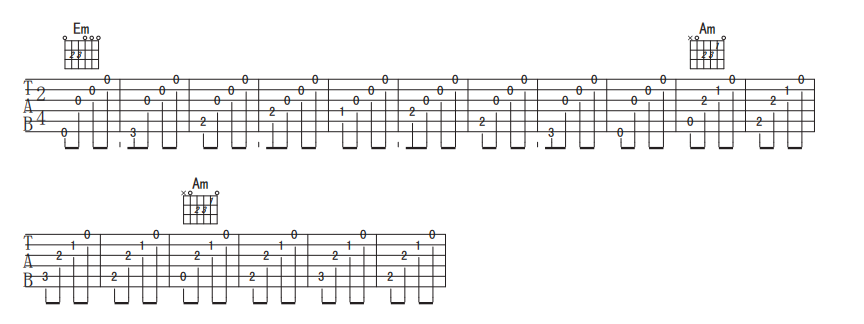
\includegraphics[width=17cm,height=10cm]{youshouAGD}
			\caption{阿瓜多右手练习琴谱}
		\end{figure}
		
		Em 6321 | Em + 6弦3品 6321 | Em 5321 | Em 4321 | Em-无名指+食指4弦1品 4321 | Em 4321 | Em 5321 | Em+6弦3品 6321 | Em 6321 |
		
		 Am 5321 | Am-中指+5弦2品 5321 | Am-中指+5弦3品 5321 | Am-中指+5弦2品 5321 | Am 5321
	
	
	\section{蜘蛛爬弦 练习}
		\begin{figure}[H]
			\centering
			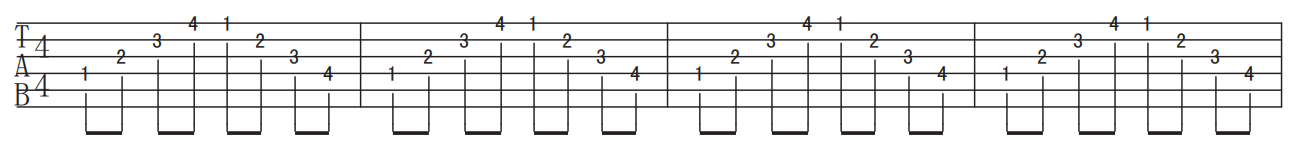
\includegraphics[width=17cm,height=4cm]{zhizhu}
			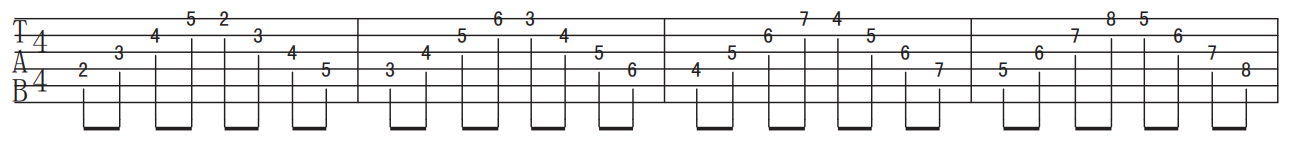
\includegraphics[width=17cm,height=4cm]{zhizhu2}
			\caption{蜘蛛左手稳定性练习}
		\end{figure}
		
	
	
	\section{滑弦 练习}
		
		\begin{figure}[H]
			\centering
			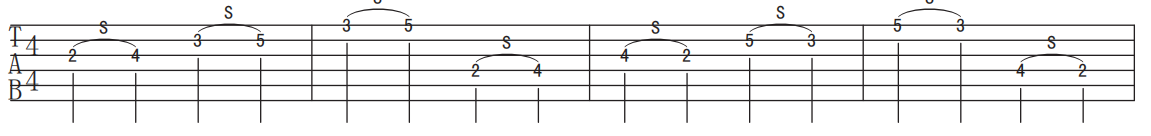
\includegraphics[width=17cm,height=4cm]{huaxian}
			\caption{从几品滑到几品}
		\end{figure}
	
	
	
	\section{击勾弦 练习}
	
	
	
	\section{半音阶 练习}
		\begin{figure}[H]
			\centering
			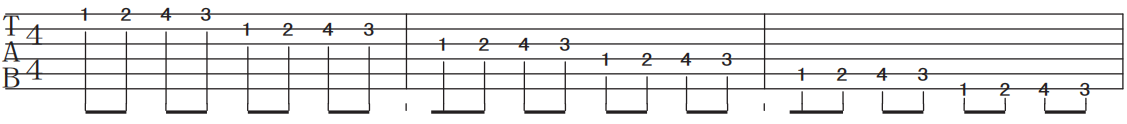
\includegraphics[width=17cm,height=3.5cm]{banyinjie}
			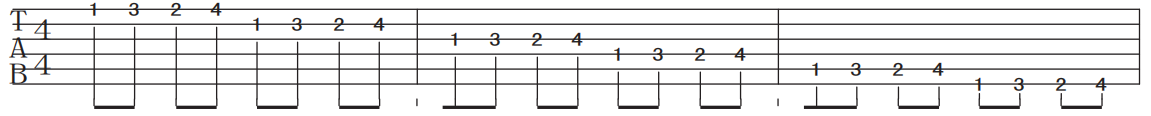
\includegraphics[width=17cm,height=3.5cm]{banyinjie1}
			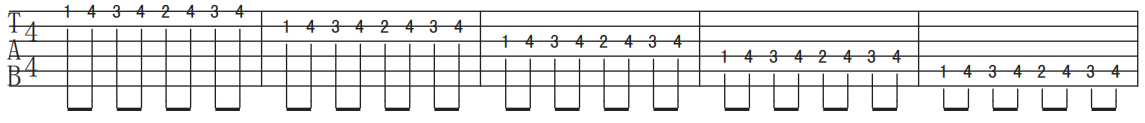
\includegraphics[width=17cm,height=3.5cm]{banyinjie2}
			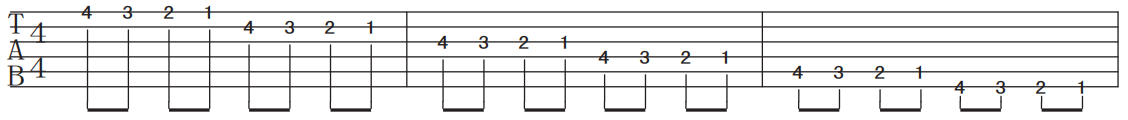
\includegraphics[width=17cm,height=3.5cm]{banyinjie3}
			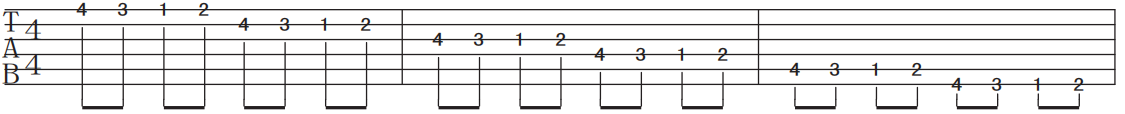
\includegraphics[width=17cm,height=3.5cm]{banyinjie4}
			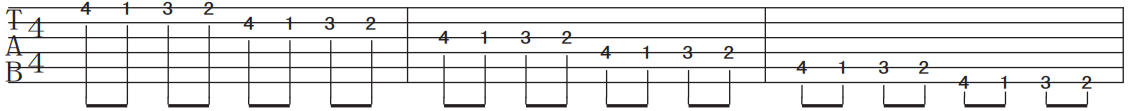
\includegraphics[width=17cm,height=3.5cm]{banyinjie5}
			\caption{半音阶6种练习}
		\end{figure}
	
	
	\section{抓拍弦 练习}
	
	
	
	\section{右手 节奏型练习}
		\begin{figure}[H]
			\centering
			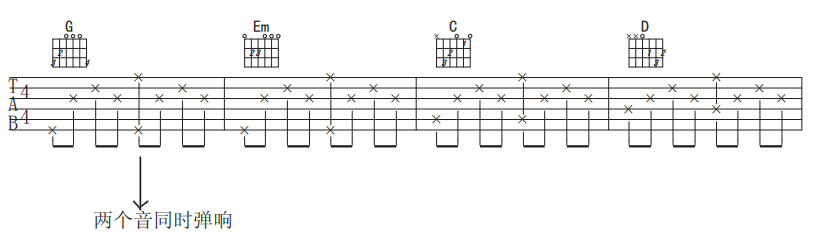
\includegraphics[width=17cm,height=5cm]{youshoujiezou}
			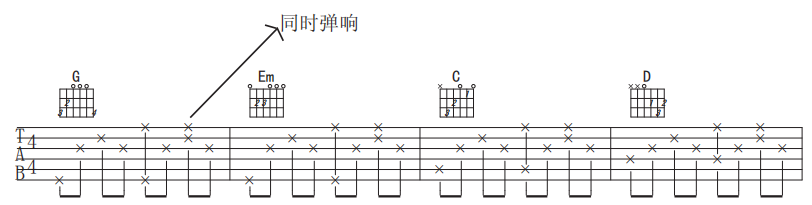
\includegraphics[width=17cm,height=5cm]{youshoujiezou1}
			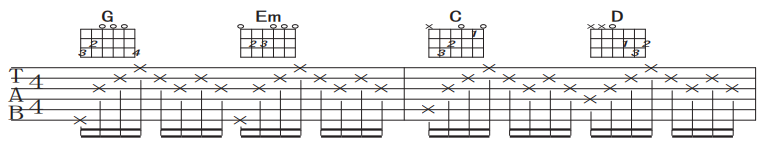
\includegraphics[width=17cm,height=5cm]{youshoujiezou2}
			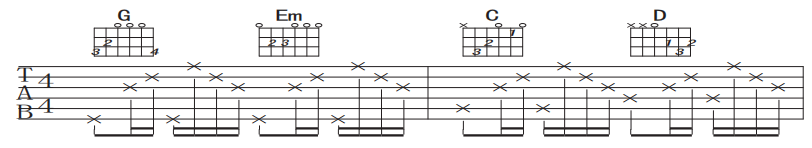
\includegraphics[width=17cm,height=5cm]{youshoujiezou3}
			\caption{右手节奏型练习}
		\end{figure}
	

	
	\section{扫弦 节奏型练习}
		\begin{figure}[H]
			\centering
			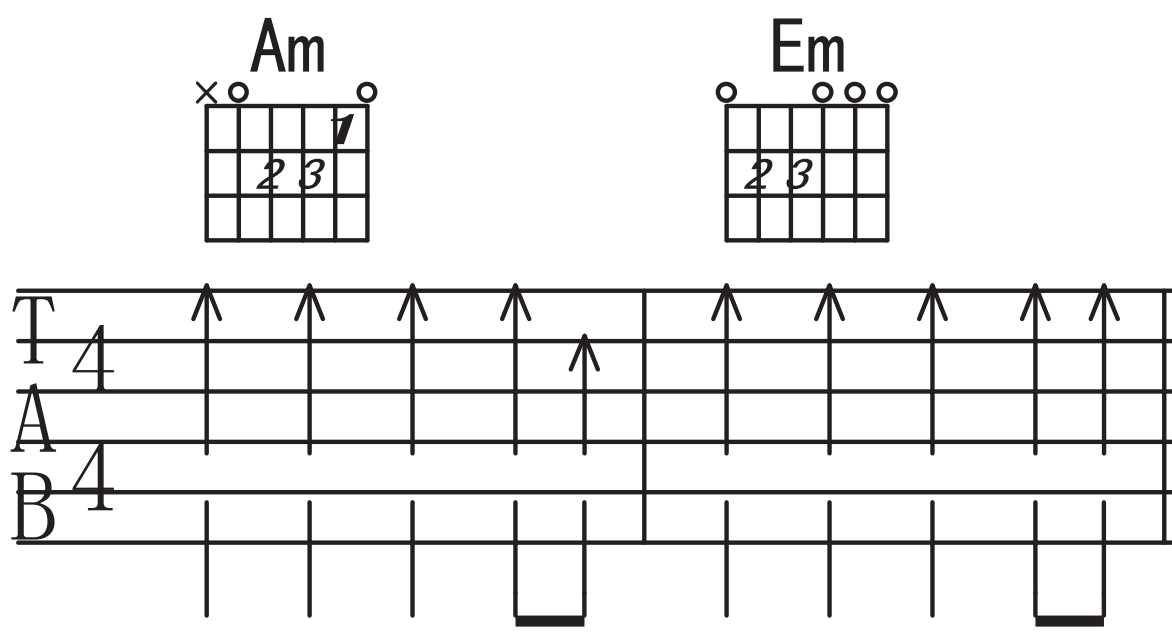
\includegraphics[width=15cm,height=6cm]{sao_01}
			\caption{扫弦节奏-前4后8}
		\end{figure}
	
	
		\begin{figure}[H]
			\centering
			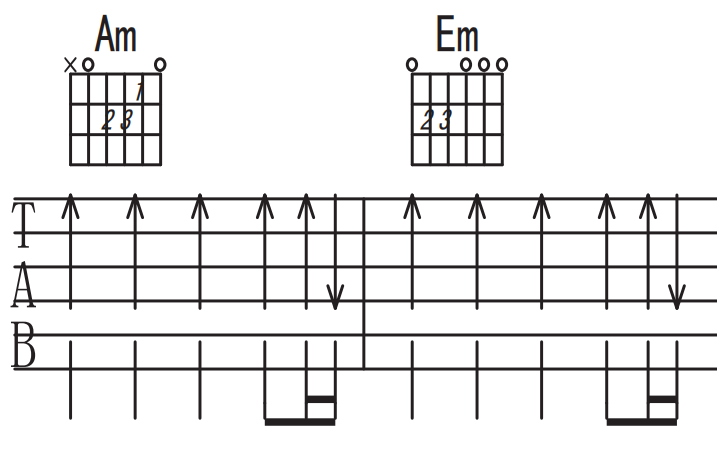
\includegraphics[width=15cm,height=6cm]{sao_02}
			\caption{扫弦节奏-前8后16}
		\end{figure}		

		\begin{figure}[H]
			\centering
			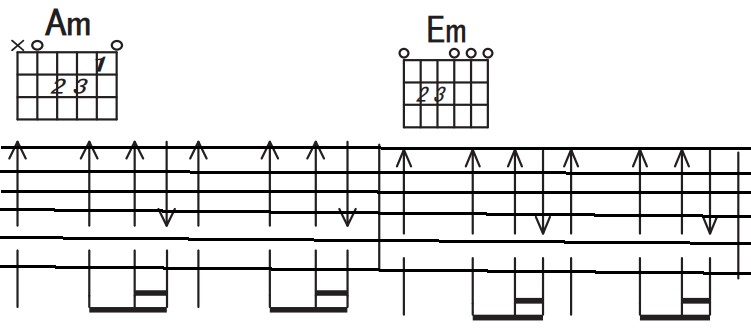
\includegraphics[width=15cm,height=6cm]{sao_03}
			\caption{扫弦节奏-double 前8后16}
		\end{figure}	
	
		\begin{figure}[H]
			\centering
			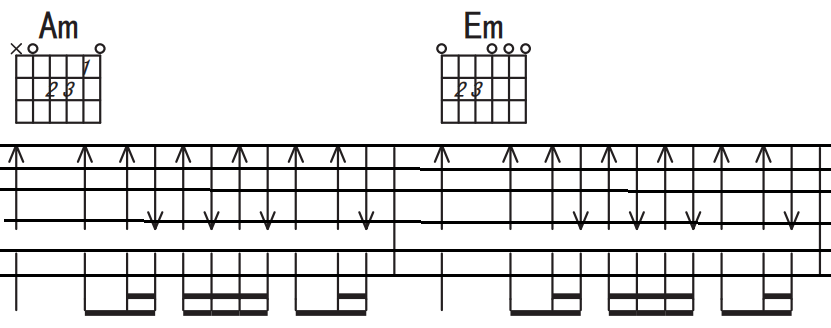
\includegraphics[width=15cm,height=6cm]{sao_04}
			\caption{扫弦节奏-前8后16 + 4个16}
		\end{figure}

\chapter{音阶、吉他技巧}
	\section{音阶}
		\url{http://blog.sina.com.cn/s/blog_498290330100qlqm.html#cmt_531ABEEB-7F000001-8764BD21-89D-8A0}
		
		\url{https://zhidao.baidu.com/question/553754625471741892.html}
		
		\subsection{Mi(3) 型音阶}
			\begin{figure}[H]
				\centering
				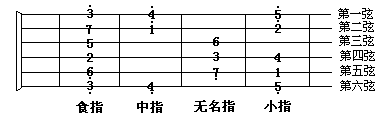
\includegraphics[width=15cm,height=6cm]{mi}
				\caption{Mi 型音阶左手按法}
			\end{figure}	
			
			Mi型音阶就是左手指按第六弦的任何一格,并将此格定为3(Mi),然后按音阶规律在这把位上形成调性音阶。
			上图中形成的是D大调音阶或Bm小调音阶。
			
			这样我们就可以推出\textbf{C调在0把位},\textbf{E调在第四把位},\textbf{G调在第七把位},\textbf{A调在第九把位}。
			
			把位确认以后,左手指法按上图,不可以跨品。我们以食指为基准就可以很轻松的弹出Mi型的音阶。	
			
			
		\subsection{So(5) 型音阶}		
			\begin{figure}[H]
				\centering
				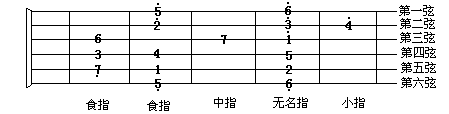
\includegraphics[width=15cm,height=6cm]{so}
				\caption{So 型音阶左手按法}
			\end{figure}	
			
			S0型音阶就是左手指按第六弦的任何一格,并将此格定为5(So),然后按音阶规律在这把位上形成调性音阶。
			上图中形成的是C大调音阶或Am小调音阶。
			
			
			这样我们就可以推出\textbf{bB调在0把位},\textbf{D调在第四把位},\textbf{F调在第七把位},\textbf{G调在第九把位}。
			
			把位确认以后,左手指法按上图,不可以跨品。我们以食指为基准就可以很轻松的弹出So型的音阶。
			练习方法同Mi型					

		
		
		\subsection{La(6) 型音阶}
			\begin{figure}[H]
				\centering
				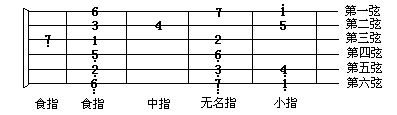
\includegraphics[width=15cm,height=6cm]{la}
				\caption{La 型音阶左手按法}
			\end{figure}	
					
			La型音阶就是左手指按第六弦的任何一格,并将此格定为6(La),然后按音阶规律在这把位上形成调性音阶。La型指法是非常重要的。
		
		
		\subsection{Si(7) 型音阶}
			\begin{figure}[H]
				\centering
				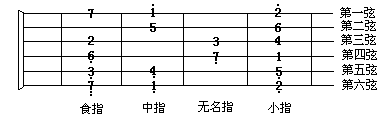
\includegraphics[width=15cm,height=6cm]{si}
				\caption{Si 型音阶左手按法}
			\end{figure}	
					
			Si型音阶就是左手指按第六弦的任何一格,并将此格定为7(Si),然后按音阶规律在这把位上形成调性音阶。
			上图中形成的是G大调音阶或Em小调音阶。
			
			这样我们就可以推出\textbf{F调在0把位},\textbf{A调在第四把位},\textbf{B调在第七把位},\textbf{D调在第九把位}。
			
			把位确认以后,左手指法按图,不可以跨品。我们以食指为基准就可以很轻松的弹出Mi型的音阶。	

		
		
		\newpage
		\subsection{各调各型音阶关联关系示例}
			\begin{figure}[H]
				\centering
				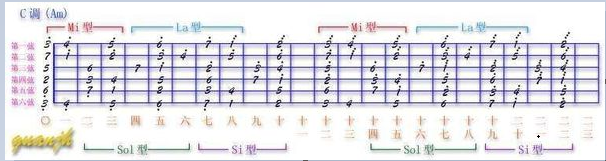
\includegraphics[width=17cm]{C}
				\caption{C 调各音阶联系示例}
			\end{figure}				
		
			\begin{figure}[H]
				\centering
				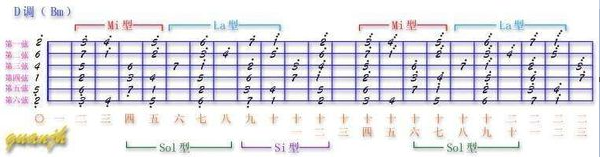
\includegraphics[width=17cm]{D}
				\caption{D 调各音阶联系示例}
			\end{figure}	
			
			\begin{figure}[H]
				\centering
				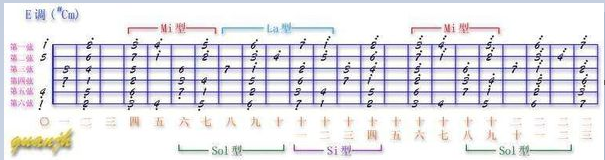
\includegraphics[width=17cm]{E}
				\caption{E 调各音阶联系示例}
			\end{figure}	
						
			\begin{figure}[H]
				\centering
				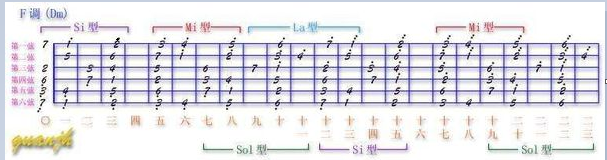
\includegraphics[width=17cm]{F}
				\caption{F 调各音阶联系示例}
			\end{figure}	

			\begin{figure}[H]
				\centering
				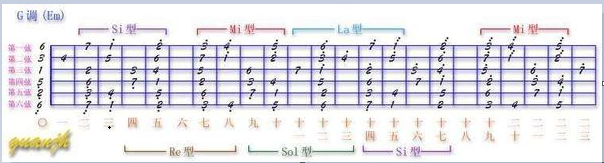
\includegraphics[width=17cm]{G}
				\caption{G 调各音阶联系示例}
			\end{figure}	

			\begin{figure}[H]
				\centering
				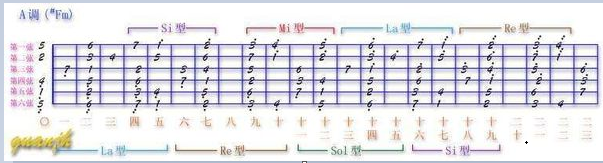
\includegraphics[width=17cm]{A}
				\caption{A 调各音阶联系示例}
			\end{figure}	
											
			\begin{figure}[H]
				\centering
				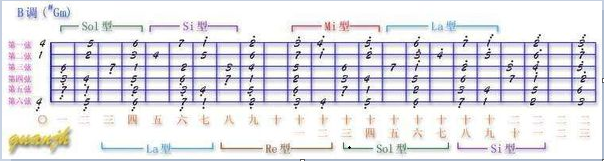
\includegraphics[width=17cm]{B}
				\caption{B 调各音阶联系示例}
			\end{figure}			
		

	
	\section{吉他和弦的CAGED系统}
	
	
	
	\section{吉他技巧}
		\subsection{击弦}
		
		\subsection{琶音}
			分解和弦逐个音弹,但是不能太慢也不能太快。
			
		\subsection{右手切音}
		
		    
\end{document} 